\documentclass[10pt]{beamer}
%%%%%%%%%%%%%%%%%%%%%%%%%%%%%%%%%%%%%%
% Metainformation
%%%%%%%%%%%%%%%%%%%%%%%%%%%%%%%%%%%%%%
\newcommand{\trauthor}{Leopold Lemmermann}
\newcommand{\trtype}{Seminar}
\newcommand{\trcourse}{Bio-inspired Artificial Intelligence}
\newcommand{\trtitle}{Image Captioning}
\newcommand{\trmatrikelnummer}{7724741}
\newcommand{\tremail}{leopold.lemmermann@studium.uni-hamburg.de}
\newcommand{\trinstitute}{Dept. Informatik -- Knowledge Technology, WTM}
\newcommand{\trwebsiteordate}{{http://www.informatik.uni-hamburg.de/WTM/}}



%%%%%%%%%%%%%%%%%%%%%%%%%%%%%%%%%%%%%%
% Languages
%%%%%%%%%%%%%%%%%%%%%%%%%%%%%%%%%%%%%%
\usepackage[english]{babel}
\selectlanguage{english}



%%%%%%%%%%%%%%%%%%%%%%%%%%%%%%%%%%%%%%
% Bind packages
%%%%%%%%%%%%%%%%%%%%%%%%%%%%%%%%%%%%%%
\usepackage{beamerthemesplit}
\usetheme{Boadilla}
%\usetheme{Copenhagen}
%\usetheme{Darmstadt}
%\usetheme{Frankfurt}
%\usetheme{Ilmenau}
%\usetheme{JuanLesPins}
%\usetheme{Madrid}
%\usetheme{Warsaw }
%\usecolortheme{dolphin}
%\setbeamertemplate{sections/subsections in toc}[sections numbered]
%\beamertemplatenavigationsymbolsempty
%\setbeamertemplate{headline}[default] 	% deaktiviert die Kopfzeile
\setbeamertemplate{navigation symbols}{}% deaktiviert Navigationssymbole
%\useinnertheme{rounded}

\usepackage{acronym}                    % Acronyms
\usepackage{algorithmic}								% Algorithms and Pseudocode
\usepackage{algorithm}									% Algorithms and Pseudocode
\usepackage{amsfonts}                   % AMS Math Packet (Fonts)
\usepackage{amsmath}                    % AMS Math Packet
\usepackage{amssymb}                    % Additional mathematical symbols
\usepackage{amsthm}
\usepackage{color}                      % Enables defining of colors via \definecolor
\usepackage{fancybox}                   % Gleichungen einrahmen
\usepackage{fancyhdr}										% Paket zur schickeren der Gestaltung der
\usepackage{graphicx}                   % Inclusion of graphics
%\usepackage{latexsym}                  % Special symbols
\usepackage{longtable}									% Allow tables over several parges
\usepackage{listings}                   % Nicer source code listings
\usepackage{lmodern}
\usepackage{multicol}										% Content of a table over several columns
\usepackage{multirow}										% Content of a table over several rows
\usepackage{rotating}										% Alows to rotate text and objects
\usepackage[section]{placeins}          % Ermoeglich \Floatbarrier fuer Gleitobj.
\usepackage[hang]{subfigure}            % Allows to use multiple (partial) figures in a fig
%\usepackage[font=footnotesize,labelfont=rm]{subfig}	% Pictures in a floating environment
\usepackage{tabularx}										% Tables with fixed width but variable rows
\usepackage{url,xspace,boxedminipage}   % Accurate display of URLs

\definecolor{uhhRed}{RGB}{254,0,0}		  % Official Uni Hamburg Red
\definecolor{uhhGrey}{RGB}{136,136,136} % Official Uni Hamburg Grey
\definecolor{uhhLightGrey}{RGB}{180,180,180} % Official Uni Hamburg LightGrey
\definecolor{uhhLightLightGrey}{RGB}{220,220,220} % Official Uni Hamburg LightLightGrey
\setbeamertemplate{itemize items}[ball]
\setbeamercolor{title}{fg=uhhRed,bg=white}
\setbeamercolor{title in head/foot}{bg=uhhRed}
\setbeamercolor{block title}{bg=uhhGrey,fg=white}
\setbeamercolor{block body}{bg=uhhLightLightGrey,fg=black}
\setbeamercolor{section in head/foot}{bg=black}
\setbeamercolor{frametitle}{bg=white,fg=uhhRed}
\setbeamercolor{author in head/foot}{bg=black,fg=white}
\setbeamercolor{author in footline}{bg=white,fg=black}
\setbeamercolor*{item}{fg=uhhRed}
\setbeamercolor*{section in toc}{fg=black}
\setbeamercolor*{separation line}{bg=black}
\setbeamerfont*{author in footline}{size=\scriptsize,series=\mdseries}
\setbeamerfont*{institute}{size=\footnotesize}

\newcommand{\opticalseperator}{0.0025\paperwidth}

\institute{Universit\"at Hamburg\\\trinstitute}
\title{\trtitle}
\subtitle{\trtype}
\author{\trauthor}
\date{}
\logo{}



%%%%%%%%%%%%%%%%%%%%%%%%%%%%%%%%%%%%%%
% Configuration
%%%%%%%%%%%%%%%%%%%%%%%%%%%%%%%%%%%%%%
\hypersetup{pdfpagemode=FullScreen}

\hyphenation{whe-ther} 									% Manually use: "\-" in a word: Staats\-ver\-trag

%\lstloadlanguages{C}                   % Set the default language for listings
\DeclareGraphicsExtensions{.pdf,.svg,.jpg,.png,.eps} % first try pdf, then eps, png and jpg
\graphicspath{{./src/}} 								% Path to a folder where all pictures are located



%%%%%%%%%%%%%%%%%%%%%%%%%%%%%%%%%%%%%%
% Custom definitions
%%%%%%%%%%%%%%%%%%%%%%%%%%%%%%%%%%%%%%
\setbeamertemplate{title page}
{
  \vbox{}
	\vspace{0.4cm}
  \begin{centering}
    \begin{beamercolorbox}[sep=8pt,center,colsep=-4bp]{title}
      \usebeamerfont{title}\inserttitle\par%
      \ifx\insertsubtitle\@empty%
      \else%
        \vskip0.20em%
        {\usebeamerfont{subtitle}\usebeamercolor[fg]{subtitle}\insertsubtitle\par}%
      \fi%
    \end{beamercolorbox}%
		\vskip0.4em
    \begin{beamercolorbox}[sep=8pt,center,colsep=-4bp,rounded=true,shadow=true]{author}
      \usebeamerfont{author}\insertauthor \\ \insertinstitute
    \end{beamercolorbox}

	  \vfill
	  \begin{beamercolorbox}[ht=8ex,center]{}
		  
\includegraphics[width=0.20\paperwidth]{res/wtmIcon.pdf}
	  \end{beamercolorbox}%
    \begin{beamercolorbox}[sep=8pt,center,colsep=-4bp,rounded=true,shadow=true]{institute}
      \usebeamerfont{institute}\trwebsiteordate
    \end{beamercolorbox}
		\vspace{-0.1cm}
  \end{centering}
}

\setbeamertemplate{frametitle}
{
\begin{beamercolorbox}[wd=\paperwidth,ht=3.8ex,dp=1.2ex,leftskip=0pt,rightskip=4.0ex]{frametitle}%
		\usebeamerfont*{frametitle}\centerline{\insertframetitle}
	\end{beamercolorbox}
	\vspace{0.0cm}
}

\setbeamertemplate{footline}
{
  \leavevmode
	\vspace{-0.05cm}
  \hbox{
	  \begin{beamercolorbox}[wd=.32\paperwidth,ht=4.8ex,dp=2.7ex,center]{author in footline}
	    \hspace*{2ex}\usebeamerfont*{author in footline}\trauthor
	  \end{beamercolorbox}%
	  \begin{beamercolorbox}[wd=.60\paperwidth,ht=4.8ex,dp=2.7ex,center]{author in footline}
	    \usebeamerfont*{author in footline}\trtitle
	  \end{beamercolorbox}%
	  \begin{beamercolorbox}[wd=.07\paperwidth,ht=4.8ex,dp=2.7ex,center]{author in footline}
	    \usebeamerfont*{author in footline}\insertframenumber{}
	  \end{beamercolorbox}
  }
	\vspace{0.15cm}
}
\renewcommand{\normalsize}{\fontsize{13.5pt}{13.5pt}\selectfont}
\renewcommand{\large}{\fontsize{15.8pt}{15.8pt}\selectfont}
\renewcommand{\Large}{\fontsize{19.0pt}{19.0pt}\selectfont}



%%%%%%%%%%%%%%%%%%%%%%%%%%%%%%%%%%%%%%
% Additional 'theorem' and 'definition' blocks
%%%%%%%%%%%%%%%%%%%%%%%%%%%%%%%%%%%%%%
\newtheorem{axiom}{Axiom}[section]
%Usage:%\begin{axiom}[optional description]%Main part%\end{fakt}

%Additional types of axioms:
\newtheorem{observation}[axiom]{Observation}

%Additional types of definitions:
\theoremstyle{remark}
\newtheorem{remark}[section]{Remark}



%%%%%%%%%%%%%%%%%%%%%%%%%%%%%%%%%%%%%%
% Abbreviations and mathematical symbols
%%%%%%%%%%%%%%%%%%%%%%%%%%%%%%%%%%%%%%
\newcommand{\modd}{\text{ mod }}
\newcommand{\RS}{\mathbb{R}}
\newcommand{\NS}{\mathbb{N}}
\newcommand{\ZS}{\mathbb{Z}}
\newcommand{\dnormal}{\mathit{N}}
\newcommand{\duniform}{\mathit{U}}

\newcommand{\erdos}{Erd\H{o}s}
\newcommand{\renyi}{-R\'{e}nyi}



%%%%%%%%%%%%%%%%%%%%%%%%%%%%%%%%%%%%%%
% Display of TOCs:
%%%%%%%%%%%%%%%%%%%%%%%%%%%%%%%%%%%%%%
% \AtBeginSection[]
% {
% 	\setcounter{tocdepth}{2}
% 	\frame
% 	{
% 	  \frametitle{Outline}
% 		\tableofcontents[currentsection]
% 	}
% }



%%%%%%%%%%%%%%%%%%%%%%%%%%%%%%%%%%%%%%
% Document
%%%%%%%%%%%%%%%%%%%%%%%%%%%%%%%%%%%%%%
\begin{document}
\renewcommand{\arraystretch}{1.2}

\begin{frame}[plain]
	\titlepage
\end{frame}

%%%%%%%%%%%%%%%%%%%%%%%%%%%%%%%%%%%%%%
% Content
%%%%%%%%%%%%%%%%%%%%%%%%%%%%%%%%%%%%%%

\begin{frame}{Introduction}
	\textbf{What is Image Captioning?}
	\begin{itemize}
		\item Task: Generate descriptive textual captions for images.
		\item Combines computer vision (CV) and natural language processing (NLP).
		\item Application examples: Assistive technology, automated metadata generation.
	\end{itemize}
\end{frame}

\begin{frame}{Introduction}
	\begin{figure}[H]
		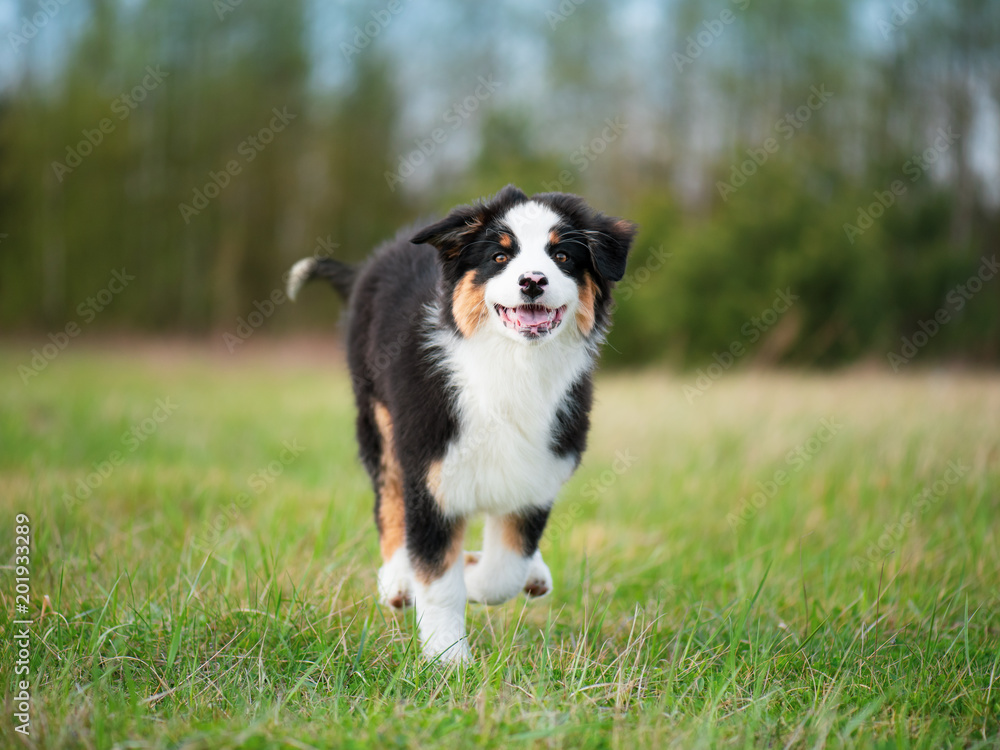
\includegraphics[width=.6\textwidth]{res/dog.jpg}
		\caption{A dog running on a field.}\label{fig:dog}
	\end{figure}
\end{frame}

\begin{frame}{Research Question}
	How do different decoder architectures (GRU, LSTM, Transformer) perform in the context of image captioning on the Flickr8k dataset?
\end{frame}

\begin{frame}{Methodology: Dataset and Features}
	\textbf{Dataset: Flickr8k}
	\begin{itemize}
		\item Contains 8,000 images with five captions per image.
	\end{itemize}
	\textbf{Feature Extraction}
	\begin{itemize}
		\item Pre-trained EfficientNet B0 model.
		\item Extracts high-level features from images.
	\end{itemize}
\end{frame}

\begin{frame}{Methodology: Decoder Architectures}
	\textbf{Architectures Evaluated}
	\begin{itemize}
		\item GRU (Gated Recurrent Units)
		\item LSTM (Long Short-Term Memory Networks)
		\item Transformer
	\end{itemize}
	\textbf{Implementation}
	\begin{itemize}
		\item Implemented in PyTorch.
		\item Trained using image features and paired captions.
	\end{itemize}
\end{frame}

\begin{frame}{Methodology: Decoder Architectures}
	\begin{figure}[H]
		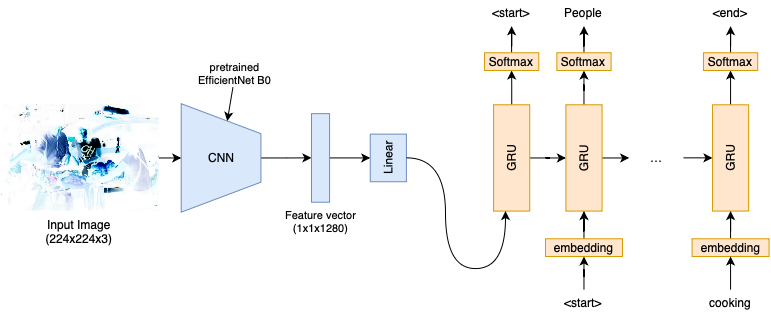
\includegraphics[width=.9\textwidth]{res/gru.png}
		\caption{GRU Decoder.}\label{fig:gru}
	\end{figure}
\end{frame}

\begin{frame}{Methodology: Decoder Architectures}
	\begin{figure}[H]
		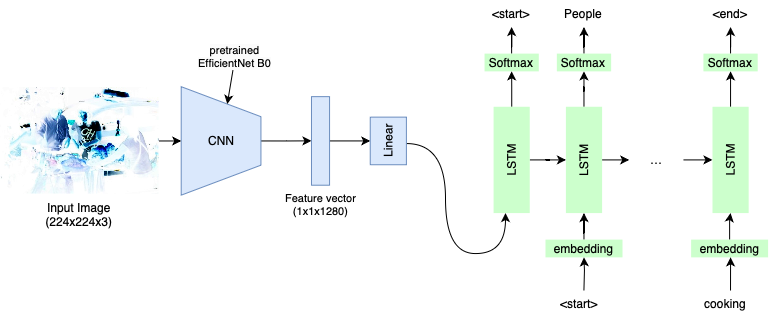
\includegraphics[width=.9\textwidth]{res/lstm.png}
		\caption{LSTM Decoder.}\label{fig:lstm}
	\end{figure}
\end{frame}

\begin{frame}{Methodology: Decoder Architectures}
	\begin{figure}[H]
		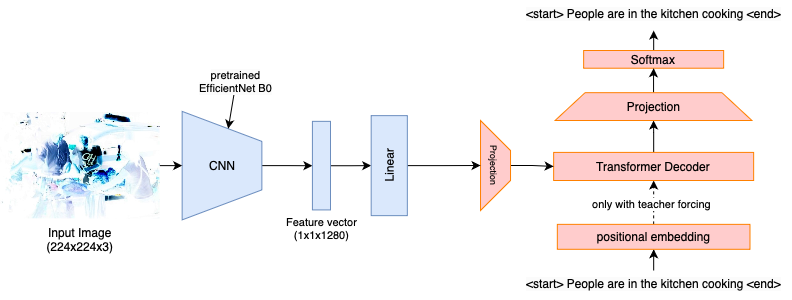
\includegraphics[width=.9\textwidth]{res/transformer.png}
		\caption{Transformer Decoder.}\label{fig:transformer}
	\end{figure}
\end{frame}

\begin{frame}{Results: Metrics}
	\textbf{Evaluation Metrics}
	\begin{itemize}
		\item BLEU: Measures n-gram overlap.
		\item METEOR: Considers semantic matching (synonyms and stemmed).
		\item NIST: Focuses on information content (rarer n-grams are weighted higher).
	\end{itemize}
\end{frame}

\begin{frame}{Results: Comparison of Architectures}
	\begin{itemize}
		\item GRU and LSTM outperform Transformer.
		\item Transformer struggles with smaller datasets like Flickr8k.
	\end{itemize}
	\textbf{Visual Comparison}
	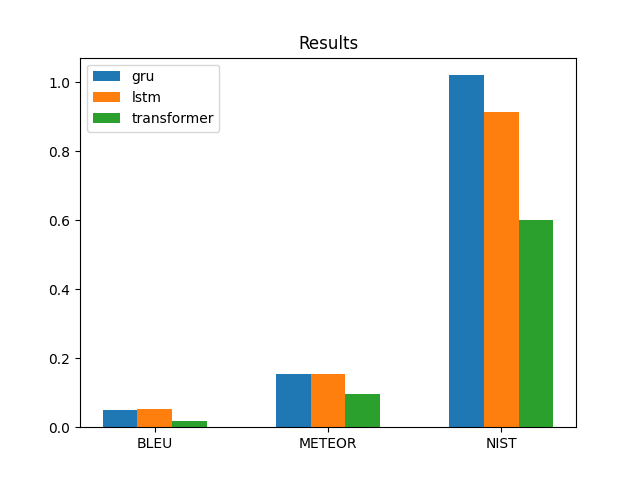
\includegraphics[width=.6\textwidth]{res/metrics.png}
\end{frame}

\begin{frame}{Discussion}
	\textbf{Insights and Implications}
	\begin{itemize}
		\item Traditional architectures (GRU, LSTM) remain competitive.
		\item Transformers may require larger datasets to realize their full potential.
	\end{itemize}
\end{frame}

\begin{frame}{Conclusion and Future Work}
	\textbf{Summary}
	\begin{itemize}
		\item Evaluated GRU, LSTM, and Transformer for image captioning.
		\item GRU and LSTM outperform Transformer on Flickr8k.
	\end{itemize}
	\textbf{Future Work}
	\begin{itemize}
		\item Test on larger datasets (e.g., MS COCO).
		\item Finetune pretrained models.
	\end{itemize}
\end{frame}

\end{document}
